\documentclass{article}

\title{ECS 252: Computer Networks \\ Assignment 5}
\author{Yuyang(Peter) Rong \\917781535 \\ PtrRong@ucdavis.edu}

\usepackage[utf8]{inputenc}
\usepackage{graphicx}
\usepackage[colorlinks,linkcolor=red]{hyperref}
\usepackage{amsmath, amsthm, amssymb}
\usepackage[shortlabels]{enumitem}
\usepackage{subfloat}
\usepackage{booktabs}
\usepackage{color}
\definecolor{mygreen}{rgb}{0,0.6,0}
\definecolor{mygray}{rgb}{0.5,0.5,0.5}
\definecolor{mymauve}{rgb}{0.58,0,0.82}

% For listings
% In case we need rust format, check https://github.com/denki/listings-rust
\usepackage{listings}
\lstset{ %
    frame=single,
    % numbers=left,
    backgroundcolor=\color{white},   % choose the background color
    basicstyle=\ttfamily\footnotesize,        % size of fonts used for the code
    breaklines=true,                 % automatic line breaking only at whitespace
    captionpos=b,                    % sets the caption-position to bottom
    commentstyle=\color{mygreen},    % comment style
    escapeinside={(*@}{@*)},         % if you want to add LaTeX within your code
    keywordstyle=\color{blue},       % keyword style
    stringstyle=\color{mymauve},     % string literal style
    tabsize=1,
    % where to put the line-numbers; possible values are (none, left, right)
    numbers = left,
    % how far the line-numbers are from the code
    numbersep = 10 pt,
    % the style that is used for the line-numbers
    numberstyle = \ttfamily,
    % the step between two line-numbers. If it's 1, each line will be numbered 
    stepnumber = 1,
}
\usepackage{ulem}
\usepackage{mathtools}

% For autoref & section reference.
\usepackage{hyperref}
\def\sectionautorefname{Section}
\def\subsectionautorefname{Section}
\def\subsubsectionautorefname{Section}


\usepackage{tikz}
\usepackage{pgfplots}
\usetikzlibrary{shapes,shapes.geometric,backgrounds,arrows,automata,positioning,cd,}
\tikzset{
    cfgedge/.style   = {black, -, >=stealth},
    thickcfgedge/.style   = {black, -, >=stealth, line width=1.1pt},
}
\usepackage{float}

\usepackage{subfigure}

\begin{document}
\maketitle


\section*{Problem 1}

\begin{figure}[H]
    \centering
    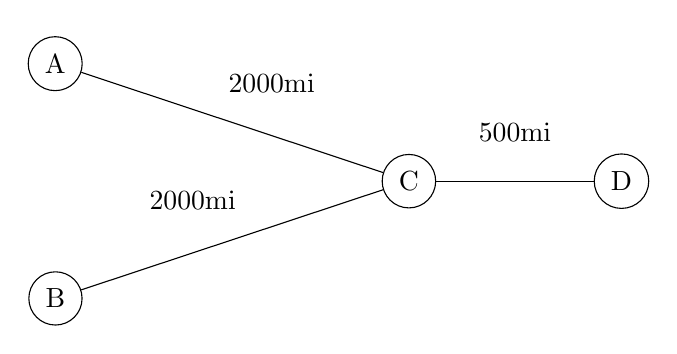
\begin{tikzpicture}[auto]
        \tikzstyle{every node} = [align=center, draw, circle]
        \node(C){C};
        \node[above left=1cm and 4cm of C](A){A};
        \node[below left=1cm and 4cm of C](B){B};
        \node[right=2cm of C](D){D};

        \path (C) edge[cfgedge] node [draw=none] {$500 \text{mi}$} (D);
        \path (A) edge[cfgedge] node [draw=none] {$2000 \text{mi}$} (C);
        \path (B) edge[cfgedge] node [draw=none] {$2000 \text{mi}$} (C);
    \end{tikzpicture}
\end{figure}

Figure shows a four node network.
$C$ receives frames from $A$ and $B$ and forwards them to $D$.
We assumethe following characteristics:

\begin{itemize}
    \item Data rate between $A$ and $C$ is $100 \text{Kbps}$.
    \item Data rate between $B$ and $C$ is $100 \text{Kbps}$.
    \item Propagation delay is $10\mu \text{sec/mile}$.
    \item The node are connected through full-duplex lines.
    \item Data frames are $1000 bits$ long.
    \item Each data frame is acknowledged and ACKs are of negligible length.
\end{itemize}

\begin{enumerate}
    \item Assuming that $C$ uses a stop-and-wait protocol to send packets to $D$, determine the data rate of the link between $C$ and $D$ so that $C$ does not get flooded given that 1) $A$ and $B$ are both using a slidingwindow protocol with a window size 2.

    \item What will be the answer to previous part if the window size between $B$ and $C$ is increased to 6.
\end{enumerate}
\subsection*{Solution}

\begin{enumerate}
    \item  Time to send one packet between $AC$: $T_{\text{send}} = 1000 \text{bit} / 100 \text{Kbps} = 10 \text{ms}$
          Single packet between $AC$:
          $T_{AC} = 10 \mu \text{sec/mile} * 2000 \text{mi} * 2 + T_{\text{send}} = 50 \text{ms}$

          Given window size of two, $C$ is receive 2 packets from $A$ every $50 \text{ms}$.
          Given link $AC$ and $BC$ are the same and they are both sending, $C$ receives 4 packets every $50 \text{ms}$.

          Since $C$ is stop-and-wait, $C$ must finish a packet in $12.5 \text{ms}$.
          The round time between $CD$ is $T_{CD} = 10 \mu \text{sec/mile} * 500 \text{mi} * 2 = 10 \text{ms}$.
          Thus the data needs to be send in $2.5 \text{ms}$, giving us a bandwidth of $1000 \text{bit} / 2.5 \text{ms} = 400 \text{Kbps}$

    \item When the window size is 12, $T_{\text{send}}$ dominates the propagation time.
          Thus $C$ is receiving 2 packets per $10 \text{ms}$, one from $A$ and one from $B$.
          Meaning that $C$ needs to send out one packet in $5 \text{ms}$, which is impossible when $C$ is stop and wait.
          This means that $C$ will always be flooded.
\end{enumerate}

\section*{Problem 2}

\subsection*{Solution}


\section*{Problem 3}

In this problem we will work through the idea of statistical multiplexing that we discussed in class.
Nodes are connected to a switch using high-bandwidth links, i.e., the links between the nodes and the switch are not
limiting.
The outgoing link form the switch is $M$ Mbps.
Consider that each node is active with probability $p$ and when it is active it transmits data at $R$ Kbps.
We define congestion when the instantaneous rate is greater than the link rate.
Write a code (Matlab, R, or Python) to answer the following questions.

\begin{enumerate}
      \item Assume that $M = 1$ Mbps, $R = 200$ Kbps, and $p = 0.2$.
            Plot the probability of congestion $P_c$ as a
            function of $N$.
      \item Repeat the previous case with $M = 1$ Mbps, $R = 800$ Kbps, and $p = 0.01$.
      \item Here we turn the problem around to answer a capacity estimation problem.
            We are given that $N = 20$,
            $R = 200$ Kbps, and $p = 0.2$.
            We are also given that the allowed probability of congestion $P_c$ is $0.1$.
            Rework the code in part (1) to find the minimum value of $M$ that is needed.
\end{enumerate}

\subsection*{Solution}


\section*{Problem 4}

In class we had derived did a simple queueing analysis to determine $\overline{N}$ which is the mean number of packets
in the system (buffer + transmitted).

\begin{enumerate}
    \item Determine the the variance of $N$?
    \item Plot (or tabulate) the mean and standard deviation $SD(N) = \sqrt{Var(N)}$ for different values of $\rho = 0.1, 0.2, \cdots , 0.9$.
    \item Why is a high value of $SD(N)$ bad for distributed networking applications?
\end{enumerate}

\subsection*{Solution}

\begin{enumerate}
    \item Given $P(N) = (1-\rho)\rho^N$, $E(N) = \frac{\rho}{1-\rho}$, we can get
          \begin{align*}
              Var(N) & = \sum_{k=0}^N (E(N) - k)^2 P(k) \\
          \end{align*}
    \item
\end{enumerate}

\end{document}
\grid
